\documentclass[a4paper,12pt]{article}

%% Definitioner för LIPS-dokument

\usepackage[english]{babel}
\usepackage[utf8]{inputenc}
\usepackage[T1]{fontenc}
\usepackage{times}
\usepackage{ifthen}

\usepackage[margin=25mm]{geometry}

\usepackage{fancyhdr}
\pagestyle{fancy}
\lhead{}
\chead{\textbf{\LIPSprojekttitel}}
\rhead{\textbf{\textsl{LiTH}}\\\textbf{\LIPSdatum}}
\lfoot{\textbf{\LIPSkursnamn}\\\textbf{\LIPSdokumentansvarig}}
\cfoot{\textbf{\LIPSprojektgrupp}\\\textbf{\LIPSgruppepost}}
\rfoot{\textbf{\textsc{Lip}s}\\\textbf{Page~\thepage}}

\setlength{\parindent}{0pt}
\setlength{\parskip}{1ex plus 0.5ex minus 0.2ex}


\newcommand{\twodigit}[1]{\ifthenelse{#1<10}{0}{}{#1}}
\newcommand{\dagensdatum}{\number\year-\twodigit{\number\month}-\twodigit{\number\day}}

%%  Redefinitions of commands containing @
\makeatletter
\makeatother

\newcommand{\LIPStitelsida}{%
{\ }\vspace{45mm}
\begin{center}
  \textbf{\Huge \LIPSdokumenttyp}
\end{center}
\begin{center}
  {\Large Editor: \LIPSredaktor}
\end{center}
\begin{center}
  {\Large \textbf{Version \LIPSversion}}
\end{center}
\vfill
\begin{center}
  {\large Status}\\[1.5ex]
  \begin{tabular}{|*{3}{p{40mm}|}}
    \hline
    Reviewed & \LIPSgranskare & \LIPSgranskatdatum \\
    \hline
    Approved & \LIPSgodkannare & \LIPSgodkantdatum \\
    \hline
  \end{tabular}
\end{center}
\newpage
}


\newenvironment{LIPSprojektidentitet}{%
{\ }\vspace{45mm}
\begin{center}
  {\Large PROJECT IDENTITY}\\[0.5ex]
  {\small
  \LIPSartaltermin, \LIPSprojektgrupp\\
  Linköping Institute of Technology, IFM
  }
\end{center}
\begin{center}
  {\small Group members}\\
%  \begin{tabular}{|p{30mm}|p{40mm}|p{35mm}|p{45mm}|}
  \begin{tabular}{|l|l|p{25mm}|l|}
    \hline
    \textbf{Name} & \textbf{Responsibility} & \textbf{Phone} & \textbf{E-mail} \\
    \hline
}%
{%
    \hline
  \end{tabular}
\end{center}
\begin{center}
  {\small
%    \textbf{E-mail for the group}: \LIPSgruppepost\\
%    \textbf{Webpage}: \LIPSgrupphemsida\\[1ex]
    \textbf{Customer}: \LIPSkund\\
    \textbf{Customer contact}: \LIPSkundkontakt\\
    \textbf{Sponsor/Course leader}: \LIPSkursansvarig\\
    \textbf{Supervisors/Experts}: \LIPShandledare\\
  }
\end{center}
\newpage
}
\newcommand{\LIPSgruppmedlem}[4]{\hline {#1} & {#2} & {#3} & {#4} \\}



\newenvironment{LIPSdokumenthistorik}{%
\begin{center}
  Version log\\[1ex]
  \begin{small}
    \begin{tabular}{|l|l|p{60mm}|l|l|}
      \hline
      \textbf{Version} & \textbf{Date} & \textbf{Performed changes} & \textbf{Performed by} & \textbf{Reviewed} \\
      }%
    {%
      \hline
    \end{tabular}
  \end{small}
\end{center}
}
\newcommand{\LIPSversionsinfo}[5]{\hline {#1} & {#2} & {#3} & {#4} & {#5} \\}

\newcounter{LIPSkravnummer}
\newcounter{LIPSunderkravnummer}[LIPSkravnummer]
\newenvironment{LIPSkravlista}{%
  \begin{tabular}{|p{25mm}|p{25mm}|p{72mm}|p{18mm}|}
    }%
  {%
    \hline
  \end{tabular}
}
\newcommand{\LIPSmilstolpe}[3]{\hline {#1} & {#2} & {#3} \\}
\newcounter{LIPSaktivitetsnummer}
\newcommand{\LIPSaktivitet}[3]{\hline\stepcounter{LIPSaktivitetsnummer}\textbf{\arabic{LIPSaktivitetsnummer}} & {#1} & {#2} & {#3} \\}

\newcommand{\LIPSkrav}[3]{\hline\stepcounter{LIPSkravnummer}\textbf{Krav nr \arabic{LIPSkravnummer}} & \textbf{{#1}} & {#2} & \textbf{{#3}} \\}
\newcommand{\LIPSunderkrav}[3]{\hline\stepcounter{LIPSunderkravnummer}\textbf{Requirement nr. \arabic{LIPSkravnummer}\Alph{LIPSunderkravnummer}} & \textbf{{#1}} & {#2} & \textbf{{#3}} \\}

\newcommand{\LIPSleverans}[4]{\hline {#1} & {#2} & {#3} & {#4} \\}


%%% Local Variables: 
%%% mode: latex
%%% TeX-master: "kravspec_mall"
%%% End: 

\usepackage{graphicx}
\usepackage{epstopdf}
\usepackage{gensymb}
\usepackage{longtable}


\newcommand{\LIPSartaltermin}{2013/HT}
\newcommand{\LIPSkursnamn}{TFYA50}

\newcommand{\LIPSprojekttitel}{Computational Physics}

\newcommand{\LIPSprojektgrupp}{Group 2}
\newcommand{\LIPSgruppepost}{}
\newcommand{\LIPSgrupphemsida}{}

\newcommand{\LIPSdokumentansvarig}{Björn Lindström}

\newcommand{\LIPSkund}{IFM at Linköping University - 581 00 Linköping - customer phone: 013-28 10 00 - fax: 013-13 75 68 - info@ifm.liu.se}
\newcommand{\LIPSkundkontakt}{Valeriu Chirita - 013-28 12 89 - vio@ifm.liu.se - office: G305}
\newcommand{\LIPSkursansvarig}{Valeriu Chirita - 013-28 12 89 - vio@ifm.liu.se - office: G305}
\newcommand{\LIPShandledare}{Daniel Edström - 013-28 66 93 - daned@ifm.liu.se - office: G432\\Davide Sangiovanni - 013-28 26 23 - davsan@ifm.liu.se - office: G426}


\newcommand{\LIPSdokumenttyp}{Final Report}
\newcommand{\LIPSredaktor}{Simon Wallin}
\newcommand{\LIPSversion}{0.1}
\newcommand{\LIPSdatum}{\dagensdatum}

\newcommand{\LIPSgranskare}{Björn Lindström}
\newcommand{\LIPSgranskatdatum}{\dagensdatum}
\newcommand{\LIPSgodkannare}{Valeriu Chirita}
\newcommand{\LIPSgodkantdatum}{}

\begin{document}

\LIPStitelsida

%% Argument till \LIPSgruppmedlem: namn, roll i gruppen, telefonnummer, epost
\begin{LIPSprojektidentitet}
	\LIPSgruppmedlem{Simon Wallin}{Project leader (PL)}{0762-30 06 65}{simwa252@student.liu.se}
	\LIPSgruppmedlem{Björn Lindström}{Documents (DOC)}{0735-33 55 98}{bjoli010@student.liu.se}
	\LIPSgruppmedlem{Johan Jönsson}{Code implementation (CI)}{0738-30 57 58}{johjo939@student.liu.se}
	\LIPSgruppmedlem{Fran\c{c}ois Vrel}{Code design (CD)}{0765-80 96 64}{fravr827@student.liu.se}
	\LIPSgruppmedlem{Mohammed Rashed}{Program operation (PO)}{0739-58 04 98}{mohra020@student.liu.se}
	\LIPSgruppmedlem{Simon Larsson}{Code test (CT)}{0707-31 16 46}{simla804@student.liu.se}
\end{LIPSprojektidentitet}

\tableofcontents{}

\newpage

%% Argument till \LIPSversionsinfo: versionsnummer, datum, ändringar, utfört av, granskat av
\addcontentsline{toc}{section}{Version log}
\begin{LIPSdokumenthistorik}
  \LIPSversionsinfo{0.1}{2013-09-27}{First draft}{Group}{DOC}
\end{LIPSdokumenthistorik}
\newpage

\section{Introduction}
A computer program for simulating the ineractions between atoms using Molecular Dynamics (MD) has been created. The program fulfills the requirements prescribed in the Project Plan and can with some limitations reproduce the real laws of physics at the microscopic level, as further specified in 2.1 General Overview.
\subsectio{Limitations}
The program has been designed for particles for which the Lennard-Jones potential is sufficient to describe the behavior.

\section{Program overview}

\subsection{General Description}

The project goal is to design, implement and operate a Molecular Dynamics (MD) program. Thus the different step had been done for he completion of the project:

\begin{itemize}
\item MD coding design flow ; 
\item correct selection and writing of code subroutines ;
\item MD program assembling ;
\item compiling, debugging and testing ;
\item operating the program ;
\item analyze results obtained with the program ;
\item assert the quality of the results.
\end{itemize}

The program coding language is C++ and has been compiled with Visual Studio 2010 \textregistered. For the visualization of the different results, Matlab R2010b \textregistered was used to draw the curve and display the atoms movements.

Our program uses the Verlet list, the Velocity Verlet algorithm and the Lennard Jones potential for the calculation.

The simulation gives the following results at the end of each simulation:

\begin{itemize}
\item Kinetic Energy ;
\item Potential Energy ;
\item Total Energy ;
\item Cohesive Energy ;
\item Mean Square Displacement (MSD) ;
\item Internal Pressure ; 
\item Temperature ; 
\item Debye Temperature ; 
\item Specific Heat ; 
\item Diffusion Coefficient.
\end{itemize}

And the time duration of the simulation as well as the average time per time step are displayed at the end of the simulation.

\subsection{Program Capabilities}

The program displays its capabilities in 4 different tab presented below.

\subsubsection{Material}

The program can simulate 38 different materials that can be chosen in the tab Material and the main materials that have been used for simulation are:

\begin{itemize}
\item Argon (Ar) ; 
\item Silver (Ag).
\end{itemize}

As a reminder, the crystal structure of each material are notified.

\subsubsection{Structure}

Once the materials has been chosen, the following parameters are displayed and can be changed in the tab Structure:

\begin{itemize}
\item Lattice constant (in \AA) ; 
\item Cutoff distance (in \AA) ;
\item Sigma (in \AA) ; 
\item Epsilon (in eV).
\end{itemize}

Then it is possible to choose the number of unit cells we want to use for the simulation in every direction, thus simulation of bulk and surface is possible.

The crystalline structure can also be chosen among the 3 coded ones:

\begin{itemize}
\item Face-centered cubic (FCC) ; 
\item Body-centered cubic (BCC);
\item Diamond (DIA).
\end{itemize}

Since Argon and Silver both have a FCC structures, it is the one that we will be used for the simulation.

\subsubsection{Calculations}

This tab allows us to control the length of the simulation and the time of data storing using:

\begin{itemize}
\item Run for \# timesteps ; 
\item Timestep size (in fs) ;
\item Start calculations after \# timesteps ; 
\item Store data every \# timesteps.
\end{itemize}

By clicking on the "Run from previous simulation" button, we can select a .txt file from which the simulation will run from by using the different material properties and atom's positions and velocities written in it.

By ticking the "Include visualisation", a file will be written containing the atoms position at different timesteps which will be used in Matlab to visualize the atom displacement.

Ticking "Thermostat" includes an Andersen thermostat for which we can choose the collision rate.

The Temperature (in K) can also be defined and the periodic boundary conditions in every direction.

\subsubsection{Results}

In order to start the simulation, we have to clicl on the button 'Start Simulation". The window on the right display a summary of the simulation choice at the beginning of the simulation.

\section{GUI}
\section{Logics}
This section will describe the ''machinery'' behind the simulations. We will
detail how we represent the system (i.e. the bulk or surface) and how we perform
the simulations from a computer science point of view (the physics is discussed
in other parts of this document).
\subsection{The atoms}
Our bulk, or surface, contains a number of individual atoms. Each atom is stored
as a separate instance of an atom class, containing (among other things) the
atom's mass, current velocity, position and acceleration.
\subsection{The Verlet List}
When we run our simulation we crate an array of Verlet Lists (one for each atom
in the bulk), where each entry is a linked list containing all the atoms inside
the verlet skin of the current atom (verlet list i in the list contains atom i
and all it's neighbours). When we update the Verlet Lists we loop through all
atoms in the bulk (or surface) and add all other atoms that are within the
Verlet Skin, in order to avoid double counting the forces acting on each atom we
only add one of the atoms to the other's Verlet List (i.e. if atoms i and j are
within each other's Verlet Skin, atom j will be added to atom j, but not the
other way around).
\subsubsection{Updating the Verlet Lists}
Since updating the Verlet Lists will be a huge time sink for the simulations
(since the update is of complexity $\Theta(N^2)$ the time required will increase
rapidly with an increasing number of atoms). It is therefore necessary to avoid
updating the Verlet Lists unnecessarily often, we have chosen to update the
Verlet Lists only when the total displacement of the two atoms that have moved
the most in the system is greater than the difference between the Verlet Skin
and the cutoff distance of the force calculations.
That is we update if (and only if)
\[
\max_{i}(\texttt{disp}_i) + \max_{i \neq j}(\texttt{disp}_j) \geq
\texttt{Verlet Skin} - \texttt{cutoff},\, \forall i = 1,\ldots, N
\]
This way, we update the Verlet Lists only when we might need to (we still update
a few times more than absolutely necessary, but this is hard to avoid).

\subsection{The Verlet Integrator}
In order to integrate the equations of motion for each atom, we need a numerical
integrator. We choose the Velocity Verlet Algorithm for our simulations since it
offers a good pay off between complexity and stability (i.e. time to perform
calculations versus accuracy of calculations). The integration is performed in
two steps. First the new positions of each atom is calculated depending on the
velocity and acceleration currently acting on the atom. In the second step the
new velocity and acceleration of each atom is calculated based on it current
position and current acceleration (all according to the Velocity Verlet
Algorithm).

Below is the Velocity Verlet algorithm
\begin{equation}
\bar{x}(t + \Delta t) = \bar{x}(t) + \bar{v}(t)\Delta t +
\frac{1}{2}\bar{a}(t)\Delta t^2
\end{equation}
\begin{equation}
\bar{v}(t + \Delta t) = \bar{v}(t) + \frac{\bar{a}(t) + \bar{a}(t+\Delta t)}{2}\Delta t
\end{equation}

\subsubsection{Calculating the Force}
Since (according to Newton) $\bar{F} = m*\bar{a}$ we need the force acting on
each atom in order to get the acceleration of each atom.

In our calculations we use the Lennard-Jones potential
\begin{equation}
V_{LJ} = 4\epsilon\left( \left(\frac{\sigma}{r}\right)^{12} - \left(
\frac{\sigma}{r} \right)^6 \right)
\end{equation}
And using the fact that 
\begin{equation}
\bar{F} = -\nabla(V)
\end{equation}
We can calculate the force acting on each atom using only it's current position.
In order to save computations we use the fact that $\bar{F}_{ij} = -
\bar{F}_{ji}$ (Newton's third law).

\section{Manual}
This section will give an introduction in how the program should and can be used. The first part discusses the setup and how to use the GUI. In the second part it discusses how to handle the output data.
	\subsection{GUI}
The GUI consists of window with four tabs. The first tab provides a list of elements that can be used for simulation as seen in fig \ref{fig:mat_tab}. Not that not all of these elements are suitable for Lennard-Jones potential. After each tom is written which crystal structure they have. To choose an element simply click it and select the next tab.
\begin{figure}[h!]
	\centering
	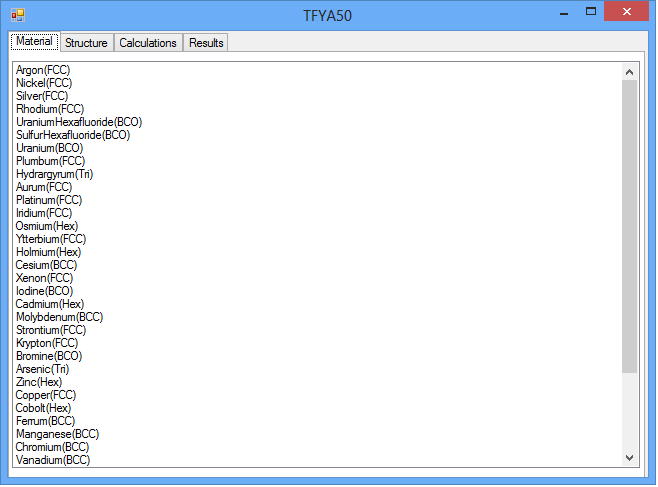
\includegraphics[width=0.7 \textwidth]{mat_tab.png}
	\caption{Interface for choosing matrial}
	\label{fig:mat_tab}
\end{figure}

Under the second tab is properties for setting up the dimensions and spacial properties of the simulation are found, see figure \ref{fig:struct_tab}. The default values, dependent on which element  that was chosen in step before, will be set here. The pre set values can be changed according to the users wishes.
\begin{figure}[h!]
	\centering
	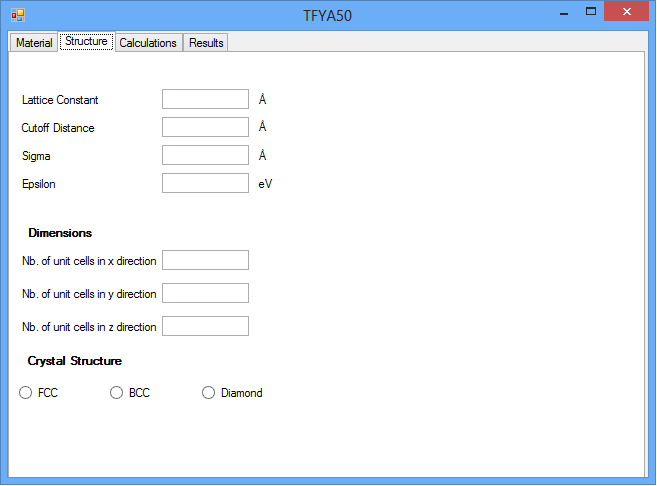
\includegraphics[width=0.7\textwidth]{struct_tab.png}
	\caption{Interface for setting material properties}
	\label{fig:struct_tab}
\end{figure}

The third tab consists of the simulation options. An overview is given in figure \ref{fig:calc_tab}. 
\begin{description}
	\item[Start calculations after \#timesteps] is the value at with point the average properties vil be started to accumulate
	\item[Run for \#timesteps] will be the amount of time steps for the simulation, tis multiplied with the timestep size will be the total runtime in femtoseconds for the simulation. 
	\item[Timestep size] will determine how long every time step should be in femtoseconds.
	\item[Include visualization] will when checked, produce a Matlab file  where the atomic movement can be seen
	\item[Save visualization every \#timestep] can be set so that not every point in the simulation is shed since that might take up to much storage space.
	\item[Save data every \#timestep] is used to decide at what interval property data should be saved.
	\item[Thermostat] will when checked activate the thermostat and an option to set the collision rate will also be given.
	\item[Collision rate] is set to a number between 0 and 1 and will be the chance of an atom colliding with the thermostat heat bath.
	\item[Temperature] is the starting temperature of the simulation. the atoms initial velocity will be scaled according to this. It will also be the temperature of the thermostat heat bath. The temperature is given in kelvin.
	\item[Use periodic boundary conditions] will when checked simulate the sample as continuous in the chosen directions. If boundary conditions are set an atom drifting away will jump over to the other side. By unchecking these conditions it is also possible to do surface simulations.
\end{description}
\begin{figure}[h!]
	\centering
	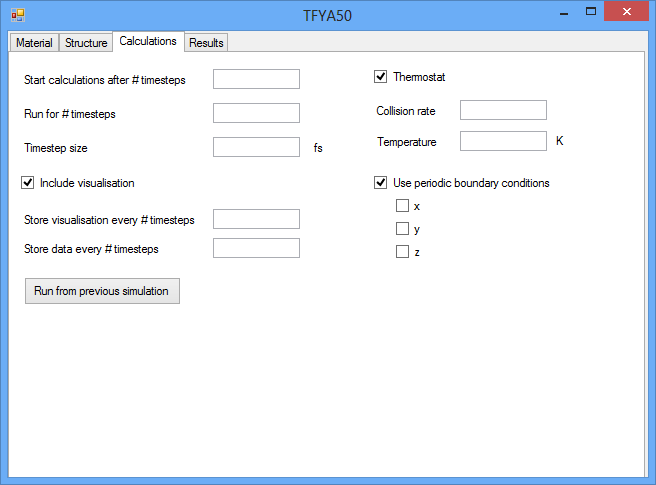
\includegraphics[width=0.7\textwidth]{calc_tab.png}
	\caption{Interface for setting calculation properties}
	\label{fig:calc_tab}
\end{figure}
	
The fourth and last tab is for starting the simulation and it will also provide the user with data on the simulation and present the average values for the listed properties when it's done as seen in figure \ref{fig:res_tab}.
\begin{figure}[h!]
	\centering
	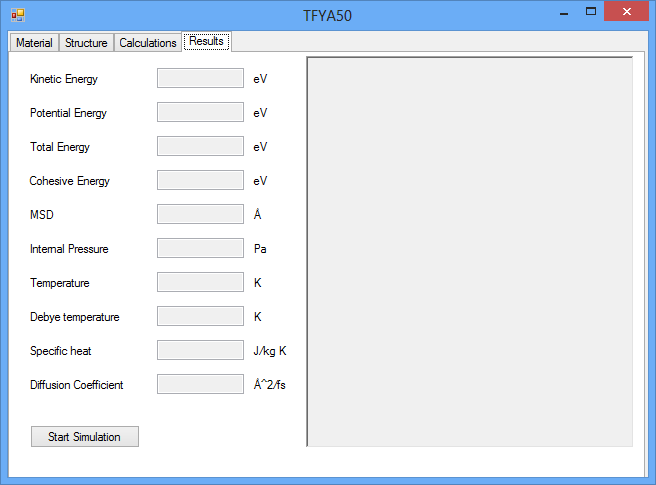
\includegraphics[width=0.7\textwidth]{res_tab.png}
	\caption{Interface for starting simulation and showing results}
	\label{fig:res_tab}
\end{figure}

When the simulation is running the program will be paused and when done a message will be send and the program will be unpaused. After running a simulation to end, a back2back file is produced to allow for multiple runs from the last state. In tab 3 simply choose run from previous simulation and choose the desired saved file.

Further more should a the user take notice and be cautious about that the program is producing new saving files with the same initial name every time it runs. This results in data being lost unless the user saves the back2back.txt, toto.txt, and titi.txt under different names or in a separate folder.

\subsection{Matlab}
Matlab is needed to produce the plots and to visualize the simulation. There are two Matlab files providing the programs that will take the data from toto.txt and titi.txt to calculate and plot the average values and the visualization respectively. To do so, launch Matlab and locate the folder with the Matlab files along with the txt files. In Matlab run the command ''plot\_data('toto.txt','\textbackslash{}t')'', where toto.txt is the name of the datafile and \textbackslash{}t is the delimiter. This allows the user to save files under different names and still being able to plot them. When running the command, nine plots will be produced. For the visualization part, simply run ''plot\_atoms()'' and the visualization will be loaded from the titi.txt file in the project folder.
\section{Simulations} 
In order to check the functionality of the program, a large number of simulations were done. The final test simulations were made with silver atoms placed in a Face-Centerd Cubi (FCC) crystal structure and were divided into two main categories, bulk simulations and surface simulations.

\subsection{Bulk Simulations}
The bulk simulations were made on a bulk of 10x10x10 unit cells, which gives a total number of 4000 atoms with the FCC structure. Periodic boundary conditions were used in all three spatial directions. 

\subsection{Surface Simulations}
The surface simulations were made on a surface of 10x10x2 unit cells, which gives a total number of 800 atoms. To obtain surface properties, periodic boundary conditions were only used in the ''x''- and ''y''-directions, but not in the ''z''-direction.

\subsection{Simulation Setup}
For all the final test simulations, both bulk and surface, on which the results presented in the next section are based on, the following settings were used:
\begin{itemize}
	\item Silver atoms
	\item FCC crystal structure
	\item Simulation starts at equilibrium (pre-simulations of 50,000 timesteps were run first to make sure that equilibrium was reached)
	\item Temperature at 500 K
	\item Time step size set to 1 fs
	\item Andersen thermostat with collision rate of 1%
	\item Each simulation ran for 50,000 time steps.
\end{itemize}

\input{results.tex}
\section{Analysis}

\subsection{Reaching equilibrium}
The system was considered to be in equilibrium

\subsection{Total and cohesive energy}
Theoretically, the total energy should be constant during the whole simulation (energy conservation). However, we can se som minor fluctruations of the value, at most 0.01 \% of the average value (See fig. \ref{totale} (it behaves the same in both bulk and surface simulations). This is most probably depending on that rounded values have to be used in the calculations. Since the fluctruations are so small after reaching equilibrium, we consider it being constant enough to run a descent simulation. 
The value of the total energy equals to the sum of the potantial and the kinetic energy, just like it should theoretically.
\subsubsection{Cohesive energy}
The cohesive energy has an average value of 1.93 eV in the main test simulation. It is hard to find any tabulated values to compare with for that temperature, so we made a test run at T=0K also. Here, the average cohesive energy was 2.34 eV, which is not the same but within a reasonable range from the tabulated value wich was found to be 2.95 eV \cite{kittel}.

\subsection{Kinetic energy and temperature}
The kinetic energy and temperature are strictly connected to eachother, which is also showed when comparing 

\subsection{Potential energy}
After reaching equilibrium, the potential energy fluctruates with less than 0.1\%. The 

\subsection{MSD and diffusion coefficient}

\subsection{Debye temperature}




% \begin{tabular}{|p{43mm}|p{15mm}|p{70mm}|p{23mm}|}
% \LIPSleverans{\textbf{Leverans}}{\textbf{Ansvarig / Godkänns av}}{\textbf{Syfte}}{\textbf{Färdig-datum}}
% \LIPSleverans{Första version av Projektplan, tidplan och systemskiss}{Simon L / Tomas}{Beskriver hur projektet ska utföras och ger en handvisning till hur roboten ska fungera}{15/2-2012}
% \LIPSleverans{Slutgiltig version av Projektplan, tidplan och systemskiss}{Simon L / Tomas}{Beskriver hur projektet ska utföras och ger en handvisning till hur konstruktionen av roboten ska ske}{23/2-2012}
% \LIPSleverans{Första version av designspecifikation}{Johan / Olov}{Visar mer detaljerat hur konstruktionen av roboten ska ske}{13/3-2012}
% \LIPSleverans{Slutgiltig version av designspecifikation}{Simon L / Olov}{Visar mer detaljerat hur konstruktionen av roboten ska ske}{16/3-2012}
% \LIPSleverans{Tidrapporter och uppdaterad tidplan}{Simon L / Tomas}{Visar hur tidfördelningen mellan de olika aktiviteterna har gått under den senaste tidsperioden, samt hur projektgruppen tänkt lägga upp sitt framtida arbete}{12/3, 19/3, 26/3, 2/4, 16/4, 23/4, 30/4, 7/5, 14/5, 21/5}
% \LIPSleverans{Statusrapport för projektet}{Simon L / Tomas}{Ger en bild av projektgruppens nuvarande status i förhållande till tidigare planering}{Vid begäran}
% \LIPSleverans{Teknisk dokumentation och användaranvisning}{Gustav / Tomas}{Ger en detaljerad bild över hur systemet fungerar, information om användargränssnit och beskrivning hur roboten används}{Tre arbetsdagar innan redovisningen vecka 20}
% \LIPSleverans{Muntlig presetation och demonstration}{Simon L / Tomas}{Slutleveransen som består av en 15-20 minuter lång presentation av robotens specifikationer och funktioner}{Vecka 20}
% \LIPSleverans{Leverans av robot}{Markus / Tomas}{En robot som uppfyller ställda krav levereras till beställaren}{vecka 20, 2012}
% \LIPSleverans{Efterstudie}{Simon L / (delges senare)}{Projektgruppen sammanställer här sina erfarenheter från projektarbetet och lämnar synpunkter på hur projektkursen skulle kunna förändras}{1/6-2012}
% \hline
% \end{tabular}




% \begin{tabular}{|p{16mm}|p{31mm}|p{100mm}|}
%         	\LIPSmilstolpe{\textbf{Namn}}{\textbf{Ansvarsområde}}{\textbf{Kommentar}}
% 	\LIPSmilstolpe{Simon L}{Projektledare}{Ansvarar för att projektgruppens sammanlagda arbete går framåt mot uppsatta mål. Uppdaterar tidsplanen och skickar in tidrapport enl. överenskommelse med beställaren}
% 	\LIPSmilstolpe{Mattias}{Dokumentansvarig}{Ansvarar för alla dokument och möteshandlingar}
% 	\LIPSmilstolpe{Gustav}{Ansvarig för reglersystem}{Huvudansvarig för robotens styr-och reglersystem}
% 	\LIPSmilstolpe{Johan}{Mjukvaruansvarig}{Ansvarar för framtagande och optimering av all programmeringskod i projektet.}
% 	\LIPSmilstolpe{Tobias}{Hårdvaruansvarig}{Ansvarar för konstruktion av nödvändig hårdvara}
% 	\LIPSmilstolpe{Simon W}{Testansvarig}{Ansvarig för att upprätta en testplan och kontinuerligt genomföra tester enligt denna}
% \hline
% \end{tabular}

% \begin{tabular}{|p{40mm}|p{20mm}|p{50mm}|p{23mm}|}
% \LIPSleverans{\textbf{Dokument}}{\textbf{Ansvarig / Godkänns av}}{\textbf{Syfte}}{\textbf{Färdig-datum}}
% \LIPSleverans{Kravspecifikation}{Simon L / Tomas}{Definierar kraven som ställs på projektet}{2/2-2012}
% \LIPSleverans{Projektplan, första inlämningnen}{Markus / Tomas}{Beskriver hur projektet ska utföras.}{15/2-2012}
% \LIPSleverans{Systemskiss, första inlämningnen}{Markus / Tomas}{Beskriver hur systemet ska byggas upp}{15/2-2012}
% \LIPSleverans{Tidplan, första inlämningnen}{Markus / Tomas}{Listar aktiviteternas budgeterade tidsåtgång.}{15/2-2012}
% \LIPSleverans{Projektplan, slutgiltig inlämning}{Simon L / Tomas}{Beskriver hur projektet ska utföras.}{23/2-2012}
% \LIPSleverans{Systemskiss, slutgiltig inlämning}{Simon L / Tomas}{Beskriver hur systemet ska byggas upp}{23/2-2012}
% \LIPSleverans{Tidplan, slutgiltig inlämning}{Simon L / Tomas}{Listar aktiviteternas budgeterade tidsåtgång.}{23/2-2012}
% \LIPSleverans{Designspecifikation, första inlämningen}{Johan / Olov}{Visar mer detaljerat hur konstruktionen av roboten ska ske}{13/3-2012}
% \LIPSleverans{Designspecifikation, slutlig inlämning}{Simon L / Olov}{Visar mer detaljerat hur konstruktionen av roboten ska ske. Version 1.0 och högre skickas till Tomas}{16/3-2012}
% \LIPSleverans{Tidrapporter och uppdaterad tidplan}{Markus / Tomas}{Visar budgeterad och spenderad tid, uppdelad på de olika aktiviteterna}{Måndagar varje vecka, med start 12/3 och slut 21/5-2012 (undantaget 9/4)}
% \LIPSleverans{Statusrapport för projektet}{Simon L / Tomas}{Dokumentet ska översiktligt sammanfatta hur projektet fortskrider.}{Vid begäran}
% \LIPSleverans{Teknisk dokumentation}{Gustav / Tomas}{Beskriver i detalj systemets uppbyggnad}{Tre arbetsdagar innan redovisningen, vecka 20}
% \LIPSleverans{Användaranvisning}{Mattias / Tomas}{Beskriver hur produkten används och dess olika funktioner.}{Tre arbetsdagar innan redovisningen, vecka 20}
% \LIPSleverans{Efterstudiedokument}{Simon L / (delges senare)}{Dokumenterar gruppens reflektioner över projektet och hur det har genomförts}{1/6-2012}
% \hline
% \end{tabular}

%%\section{Utvecklingsmetodik}

% \begin{tabular}{|p{7mm}|p{117mm}|p{23mm}|}
%         	\LIPSmilstolpe{\textbf{Nr}}{\textbf{Beskrivning}}{\textbf{Datum}}
% 	\LIPSmilstolpe{1}{Designspecifikationen accepterad av handledaren}{2012-03-16}
% 	\LIPSmilstolpe{2}{Bussen fungerar som den ska}{2012-03-23}
% 	\LIPSmilstolpe{3}{Data och mätvärden skickas via komunikationsenheten}{2012-04-30}
% 	\LIPSmilstolpe{4}{Roboten kan upptäcka korsningar}{2012-04-19}
% 	\LIPSmilstolpe{5}{Korrekt sensorinfo visas på PCn}{2012-04-20}
% 	\LIPSmilstolpe{6}{Motorn regleras autonomt utifrån sensorvärdena}{2012-04-27}
% 	\LIPSmilstolpe{7}{Styrkommandon utförs korrekt}{2012-05-04}
% \hline
% \end{tabular}

% \begin{tabular}{|p{7mm}|p{117mm}|p{23mm}|}
%         	\LIPSmilstolpe{\textbf{BP}}{\textbf{Beskrivning}}{\textbf{Datum}}
% 	\LIPSmilstolpe{BP0}{Godkännande av projektdirektiv, beslut att starta förstudie}{2012-01-20}
% 	\LIPSmilstolpe{BP1}{Godkännande av kravspecifikation, beslut att starta förberedelsefasen}{2012-02-02}
% 	\LIPSmilstolpe{BP2}{Godkännande av projektplanering, beslut att starta utförandefasen}{2012-02-23}
% 	\LIPSmilstolpe{BP3}{Godkännande av designspecifikation, beslut att fortsätta utförandefasen}{2012-03-16}
% 	\LIPSmilstolpe{BP4}{Ej specifierad}{-}
% 	\LIPSmilstolpe{BP5}{Godkännande av produktens funktionalitet, beslut att leverera}{vecka 19}
% 	\LIPSmilstolpe{BP6}{Godkännande av leverans, beslut att upplösa projektgruppen}{2012-06-01}
% \hline
% \end{tabular}

% \begin{longtable}{|p{7mm}|p{90mm}|p{23mm}|p{23mm}|}
% 	\LIPSleverans{\textbf{Nr}}{\textbf{Beskrivning}}{\textbf{Beroende av aktivitet nr}}{\textbf{Beräknad tid (h)}} 
% \LIPSaktivitet{Färdigställande av
% designspec}{}{44} 
% %% SENSOR
% 	\LIPSaktivitet{Omvandling av analoga signaler till
% digitala sådana}{}{12} 
% 	\LIPSaktivitet{Trösklande av
% sensorvärden}{2}{4} 
% 	\LIPSaktivitet{Hitt skillnaden mellan önskade och
% aktuella värden}{3}{4} 
% 	\LIPSaktivitet{Skicka skilnaden till styrenheten (via
% kommunikationsenheten)}{4 \& 10}{14} 
% 	\LIPSaktivitet{Skicka avstånd i cm till display- och
% kommunikationsenheten}{2 \& 10}{12} 
% 	\LIPSaktivitet{Upptäck
% riktningsmarkeringar}{1 \& 2}{20} 
% 	\LIPSaktivitet{Hantera
% riktningsmarkeringar}{6}{20} 
% 	\LIPSaktivitet{Upptäck korsningar}{2 \&
% 3}{20} 
% %% KOMMUNIKATION
% 	\LIPSaktivitet{Ordna master som sköter
% buss}{}{50} 
% 	\LIPSaktivitet{Skicka styrinfo till
% pc}{15 \& 23 \& 10}{15} 
% 	\LIPSaktivitet{Skicka sensorinfo till
% pc}{5 \& 15 \& 23}{15} 
% 	\LIPSaktivitet{Ta emot styrkommandon från
% pc}{15 \& 23}{15} 
% 	\LIPSaktivitet{Skicka styrkommando till styrenhet
% från kommunikqtionsenhet}{10}{15} 
% 	\LIPSaktivitet{Fixa blåtand i
% kommunikationsenhet}{}{25} 
% %% STYRENHET
% 	\LIPSaktivitet{Ta emot sensorvärden
% (Styrenhet)}{10 \& 5}{20} 
% 	\LIPSaktivitet{Reglera motorer utifrånsensorvärden}{16 \& 19 \& 22}{40} 
% 	\LIPSaktivitet{Ta emot styrkommandon
% (styrenheten)från kommunikationsenheten}{10 \& 24 \& 14}{20} 
% 	\LIPSaktivitet{Styra motorer (autonomt och manuellt)}{}{40} 
% 	\LIPSaktivitet{Skicka styrinfo till
% kommunikationsenheten från
% styrenheten}{10}{20} 
% 	\LIPSaktivitet{Hantera
% specialkommandon}{8 \& 19}{30}
% 	\LIPSaktivitet{Regulator}{5}{30} 
% %% PC 
% 	\LIPSaktivitet{Fixa blåtand i
% pc}{}{25} 
% 	\LIPSaktivitet{Hämta och skicka styrkommandon från
% pc till kommunikationsenheten (Mjukvara)}{15 \& 23}{30} 
% 	\LIPSaktivitet{Ta emot styrinfo i PC från
% kommunikationsenheten}{15 \& 23 \& 20}{20} 
% 	\LIPSaktivitet{Ta emot sensorinfo}{15 \& 23 \&
% 6}{20} 
% 	\LIPSaktivitet{Visa styrinfo på
% skärm}{25}{2} 
% 	\LIPSaktivitet{Visa sensorinfo på
% skärm}{26}{2} 
% 	\LIPSaktivitet{Ordna gränssnitt på
% pc}{}{15} 
% %% MONTERING OCH TEST
% 	\LIPSaktivitet{Montering av
% avståndssensorer}{}{10} 
% 	\LIPSaktivitet{Montering av
% linjesensorer}{}{10}
% 	\LIPSaktivitet{Montering}{30 \&
% 31}{20} 
% 	\LIPSaktivitet{Utför styrkommandon}{18 \&
% 21}{30} 
% 	\LIPSaktivitet{Test av hela systemet}{2-33 \& (35)}{35} 
% 	\LIPSaktivitet{Kalibrering av
% sensorer}{}{20}
% 	\LIPSaktivitet{Planering och utförande av tester}{}{10}
% 	\LIPSaktivitet{Test av bussen}{}{10}
% 	\LIPSaktivitet{Test av kommunikationsenheten}{}{10}
% 	\LIPSaktivitet{Test av sensorenheten}{}{10}
% 	\LIPSaktivitet{Test av styrenheten}{}{10}
% %% EFTERARBETE OCH DOKUMENTATION
% 	\LIPSaktivitet{Sammanställa och granska
% teknisk dokumentation}{samtliga}{20} 
% 	\LIPSaktivitet{Sammanställa och granska
% Användarmanual}{37}{20} 
% 	\LIPSaktivitet{Förbereda
% redovisning}{38}{15} 
% 	\LIPSaktivitet{Tidsloggning (ska ske
% kontinuerligt)}{}{20} 
% 	\LIPSaktivitet{Efterstudie}{39}{15}  
% 	\LIPSaktivitet{Rest / Reservtid}{}{46}
% 	\LIPSaktivitet{Möten}{}{70} 
% 
% \hline
% \end{longtable}
\newpage

\addcontentsline{toc}{section}{References}
\begin{thebibliography}{99}
\bibitem{lipskompendiet}\textit{Projektmodellen LIPS - } Svensson, Tomas
\\Studentlitteratur, 2011.
\end{thebibliography}
\newpage

\appendix
\section{Appendix}
\label{LetterOA}

\subsection{}
%\begin{figure}[h]
%	\centering
%	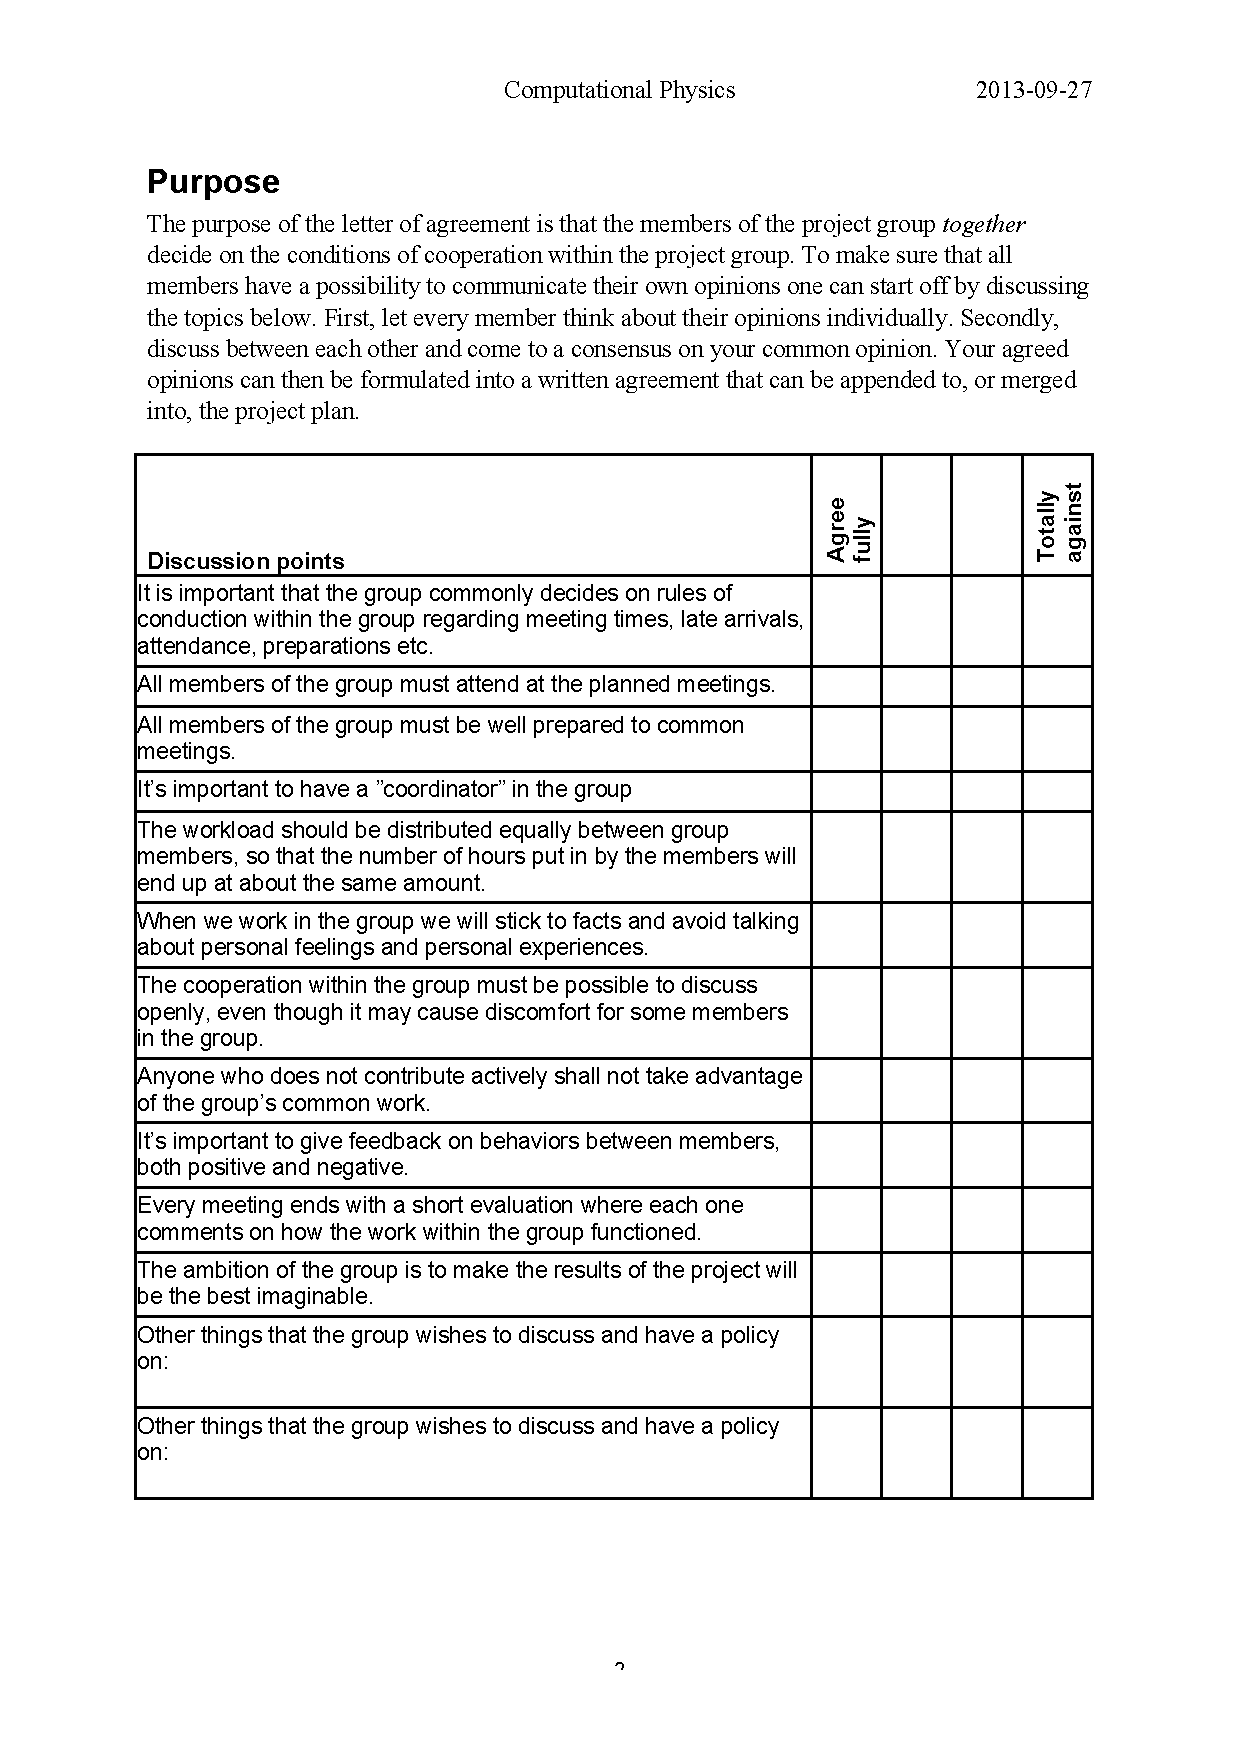
\includegraphics[trim=5mm 5mm 5mm 5mm, clip=true, scale=0.6]{Images/Letterofagreement.pdf}
%\end{figure}

\end{document} 

%%% Local Variables: 
%%% mode: latex
%%% TeX-master: t
%%% End: 

